\documentclass[journal,12pt,twocolumn]{IEEEtran}

\usepackage{setspace}
\usepackage{gensymb}


\singlespacing

\usepackage[cmex10]{amsmath}
%\usepackage{amsthm}
%\interdisplaylinepenalty=2500
%\savesymbol{iint}
%\usepackage{txfonts}
%\restoresymbol{TXF}{iint}
%\usepackage{wasysym}
\usepackage{amsthm}

\usepackage{mathrsfs}
\usepackage{txfonts}
\usepackage{stfloats}
\usepackage{bm}
\usepackage{cite}
\usepackage{cases}
\usepackage{subfig}

\usepackage{longtable}
\usepackage{multirow}

\usepackage{enumitem}
\usepackage{mathtools}
\usepackage{steinmetz}
\usepackage{tikz}
\usepackage{circuitikz}
\usepackage{verbatim}
\usepackage{tfrupee}
\usepackage[breaklinks=true]{hyperref}

\usepackage{tkz-euclide} %loads TikZ and tkz-base

\usetikzlibrary{calc,math}
\usepackage{listings}
    \usepackage{color}                                          
    \usepackage{array}                                          
    \usepackage{longtable}                                      
    \usepackage{calc}                                           
    \usepackage{multirow}                                       
    \usepackage{hhline}                                         
    \usepackage{ifthen}
    \usepackage{lscape}     
\usepackage{multicol}
\usepackage{chngcntr}

\DeclareMathOperator*{\Res}{Res}

\renewcommand\thesection{\arabic{section}}
\renewcommand\thesubsection{\thesection.\arabic{subsection}}
\renewcommand\thesubsubsection{\thesubsection.\arabic{subsubsection}}

\renewcommand\thesectiondis{\arabic{section}}
\renewcommand\thesubsectiondis{\thesectiondis.\arabic{subsection}}
\renewcommand\thesubsubsectiondis{\thesubsectiondis.\arabic{subsubsection}}

\hyphenation{op-tical net-works semi-conduc-tor}
\def\inputGnumericTable{}                                 %%

\lstset{
%language=C,
frame=single, 
breaklines=true,
columns=fullflexible
}

\begin{document}

\newtheorem{theorem}{Theorem}[section]
\newtheorem{problem}{Problem}
\newtheorem{proposition}{Proposition}[section]
\newtheorem{lemma}{Lemma}[section]
\newtheorem{corollary}[theorem]{Corollary}
\newtheorem{example}{Example}[section]
\newtheorem{definition}[problem]{Definition}

\newcommand{\BEQA}{\begin{eqnarray}}
\newcommand{\EEQA}{\end{eqnarray}}
\newcommand{\define}{\stackrel{\triangle}{=}}

\bibliographystyle{IEEEtran}

\providecommand{\mbf}{\mathbf}
\providecommand{\pr}[1]{\ensuremath{\Pr\left(#1\right)}}
\providecommand{\qfunc}[1]{\ensuremath{Q\left(#1\right)}}
\providecommand{\sbrak}[1]{\ensuremath{{}\left[#1\right]}}
\providecommand{\lsbrak}[1]{\ensuremath{{}\left[#1\right.}}
\providecommand{\rsbrak}[1]{\ensuremath{{}\left.#1\right]}}
\providecommand{\brak}[1]{\ensuremath{\left(#1\right)}}
\providecommand{\lbrak}[1]{\ensuremath{\left(#1\right.}}
\providecommand{\rbrak}[1]{\ensuremath{\left.#1\right)}}
\providecommand{\cbrak}[1]{\ensuremath{\left\{#1\right\}}}
\providecommand{\lcbrak}[1]{\ensuremath{\left\{#1\right.}}
\providecommand{\rcbrak}[1]{\ensuremath{\left.#1\right\}}}
\theoremstyle{remark}
\newtheorem{rem}{Remark}
\newcommand{\sgn}{\mathop{\mathrm{sgn}}}
\providecommand{\abs}[1]{\left\vert#1\right\vert}
\providecommand{\res}[1]{\Res\displaylimits_{#1}} 
\providecommand{\norm}[1]{\left\lVert#1\right\rVert}
%\providecommand{\norm}[1]{\lVert#1\rVert}
\providecommand{\mtx}[1]{\mathbf{#1}}
\providecommand{\mean}[1]{E\left[ #1 \right]}
\providecommand{\fourier}{\overset{\mathcal{F}}{ \rightleftharpoons}}
%\providecommand{\hilbert}{\overset{\mathcal{H}}{ \rightleftharpoons}}
\providecommand{\system}{\overset{\mathcal{H}}{ \longleftrightarrow}}
	%\newcommand{\solution}[2]{\textbf{Solution:}{#1}}
\newcommand{\solution}{\noindent \textbf{Solution: }}
\newcommand{\cosec}{\,\text{cosec}\,}
\providecommand{\dec}[2]{\ensuremath{\overset{#1}{\underset{#2}{\gtrless}}}}
\newcommand{\myvec}[1]{\ensuremath{\begin{pmatrix}#1\end{pmatrix}}}
\newcommand{\mydet}[1]{\ensuremath{\begin{vmatrix}#1\end{vmatrix}}}

\numberwithin{equation}{subsection}

\makeatletter
\@addtoreset{figure}{problem}
\makeatother

\let\StandardTheFigure\thefigure
\let\vec\mathbf

\renewcommand{\thefigure}{\theproblem}

\def\putbox#1#2#3{\makebox[0in][l]{\makebox[#1][l]{}\raisebox{\baselineskip}[0in][0in]{\raisebox{#2}[0in][0in]{#3}}}}
     \def\rightbox#1{\makebox[0in][r]{#1}}
     \def\centbox#1{\makebox[0in]{#1}}
     \def\topbox#1{\raisebox{-\baselineskip}[0in][0in]{#1}}
     \def\midbox#1{\raisebox{-0.5\baselineskip}[0in][0in]{#1}}
\vspace{3cm}

\title{Assignment 4}
\author{Surbhi Agarwal}

\maketitle

\newpage

%\tableofcontents

\bigskip

\renewcommand{\thefigure}{\theenumi}
\renewcommand{\thetable}{\theenumi}

\begin{abstract}
This document finds the equation of tangent to the circle which is parallel to another given line.
\end{abstract}

Download all python codes from 
%
\begin{lstlisting}
https://github.com/surbhi0912/EE5609/
\end{lstlisting}
%
and latex-tikz codes from 
%
\begin{lstlisting}
https://github.com/surbhi0912/EE5609/
\end{lstlisting}
%
\section{Problem}
Find the equations of the tangents to the circle
\begin{align}\nonumber
    \vec{x}^T\vec{x} -\myvec{4 & 3}\vec{x}+5 = 0
\end{align}
that are parallel to the line
\begin{align}\nonumber
    \myvec{1 & 1}\vec{x} = 0
\end{align}
\section{Solution}
The given equation of the circle is
\begin{align}\label{eq:e1}
    \vec{x}^T\vec{x} -\myvec{4 & 3}\vec{x}+5 = 0
\end{align}
Comparing this to the general second degree equation,
\begin{align}
%    \vec{x}^T\vec{V}\vec{x} + 2\vec{u}^T\vec{x} + f = 0
    \vec{V} = \vec{I}, \quad \vec{u} = \myvec{-2 \\ \frac{-3}{2}}, \quad f = 5 \label{eq:Vufvals}
\end{align}
Tthe centre $\vec{c}$ and radius $r$ are given by
\begin{align}
    \vec{c} = -\vec{u} = \myvec{2 \\ \frac{3}{2}}, r = \sqrt{\vec{u}^T\vec{u} - f} = \frac{\sqrt{5}}{2}
\end{align}
The equation of the given line is
\begin{align}
    \myvec{1 & 1}\vec{x} = 0
    \intertext{Comparing with standard equation of a line $\vec{n}^T\vec{x} = c$,}
    \vec{n}^T = \myvec{1 & 1}\\
    \implies\vec{n} = \myvec{1 \\ 1}
\end{align}
Since the tangent is parallel to this line, it's normal vector is parallel to the normal vector of the given line.
\begin{align}
    \implies\vec{n} = \myvec{1 \\ 1} \label{eq:nval}
    \intertext{And its direction vector $\vec{m}$ is given by}
    \vec{n}^T\vec{m} = 0\\
    \implies \myvec{1 & 1}\vec{m} = 0\\
    \implies \vec{m} = \myvec{1 \\-1}
\end{align}
So, the equation for the tangent can be written as:
\begin{align}
    L : \vec{x} = \vec{q} + \lambda\vec{m}
\end{align}
The point of contact $\vec{q}$ is given as
\begin{align}
    \vec{q} = \kappa\vec{n} - \vec{u}
    \intertext{where,}
    \kappa = \pm\sqrt{\frac{\vec{u}^T\vec{u} - f}{\vec{n}^T\vec{n}}} \label{eq:kappa}
\end{align}
Substituting values from \eqref{eq:Vufvals} and \eqref{eq:nval} into \eqref{eq:kappa}
\begin{align}
    \kappa = \pm\frac{\sqrt{5}}{2\sqrt{2}} \label{eq:kappaval}
    \intertext{Substituting values from \eqref{eq:Vufvals}, \eqref{eq:nval}, \eqref{eq:kappaval}}
    \vec{q} = \pm\frac{\sqrt{5}}{2\sqrt{2}}\myvec{1 \\ 1} - \myvec{-2 \\ \frac{-3}{2}}\\
    \vec{q}_1 = \frac{1}{2}\myvec{\sqrt{\frac{5}{2}}+4\\\sqrt{\frac{5}{2}}+3}\\
    \vec{q}_2 = \frac{1}{2}\myvec{-\sqrt{\frac{5}{2}}+4\\-\sqrt{\frac{5}{2}}+3}
\end{align}
From this, we get the equation of tangent is
\begin{align}
    (\vec{V}\vec{q}+\vec{u})^T\vec{x}+\vec{u}^T\vec{q}+f=0\qquad\text{Here $\vec{V} = I$}\\
    \intertext{Substituting $\vec{q} = \kappa\vec{n}-\vec{u}$}
    (\kappa\vec{n}-\vec{u}+\vec{u})^T\vec{x} + \vec{u}^T(\kappa\vec{n}-\vec{u}) + f = 0\\
    \implies \kappa\vec{n}^T\vec{x} + \kappa\vec{u}^T\vec{n} - \vec{u}^T\vec{u}+f = 0\\
    \intertext{Substituing values from \eqref{eq:Vufvals}, \eqref{eq:nval} and \eqref{eq:kappaval}, we get the equation of the tangents as :}
    \myvec{1 & 1}\vec{x} = \frac{7+\sqrt{10}}{2}
    \intertext{and}
    \myvec{1 & 1}\vec{x} = \frac{7-\sqrt{10}}{2}
\end{align}
\renewcommand{\thefigure}{1}
\begin{figure}[h!]
    \centering
    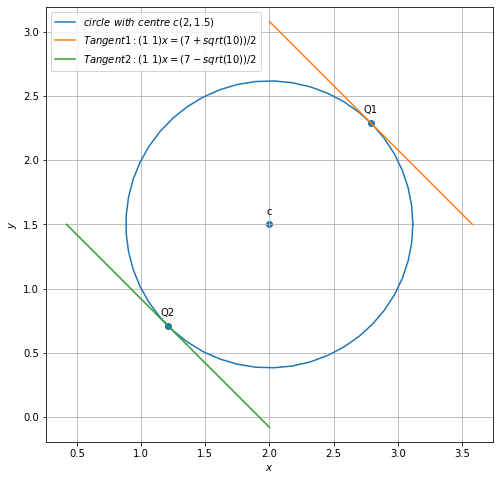
\includegraphics[width=\columnwidth]{assignment4circle.png}
    \caption{Tangents to a given circle that are parallel to the line (1 1)x = 0}
    \label{fig:fig1}
\end{figure}
\end{document}